\documentclass[10pt]{homeworg}

\usepackage{bm}
\title{Homework 2}
\author{Kevin Yang - 50244152}


\begin{document}

\maketitle

\Huge{Link to repo:}\\
\Large{https://github.com/keviny2/CPSC532W-Assignments/tree/main/HW2}


\section{Code Snippets}
\subsection{evaluation\_based\_sampling.py}

\begin{center}
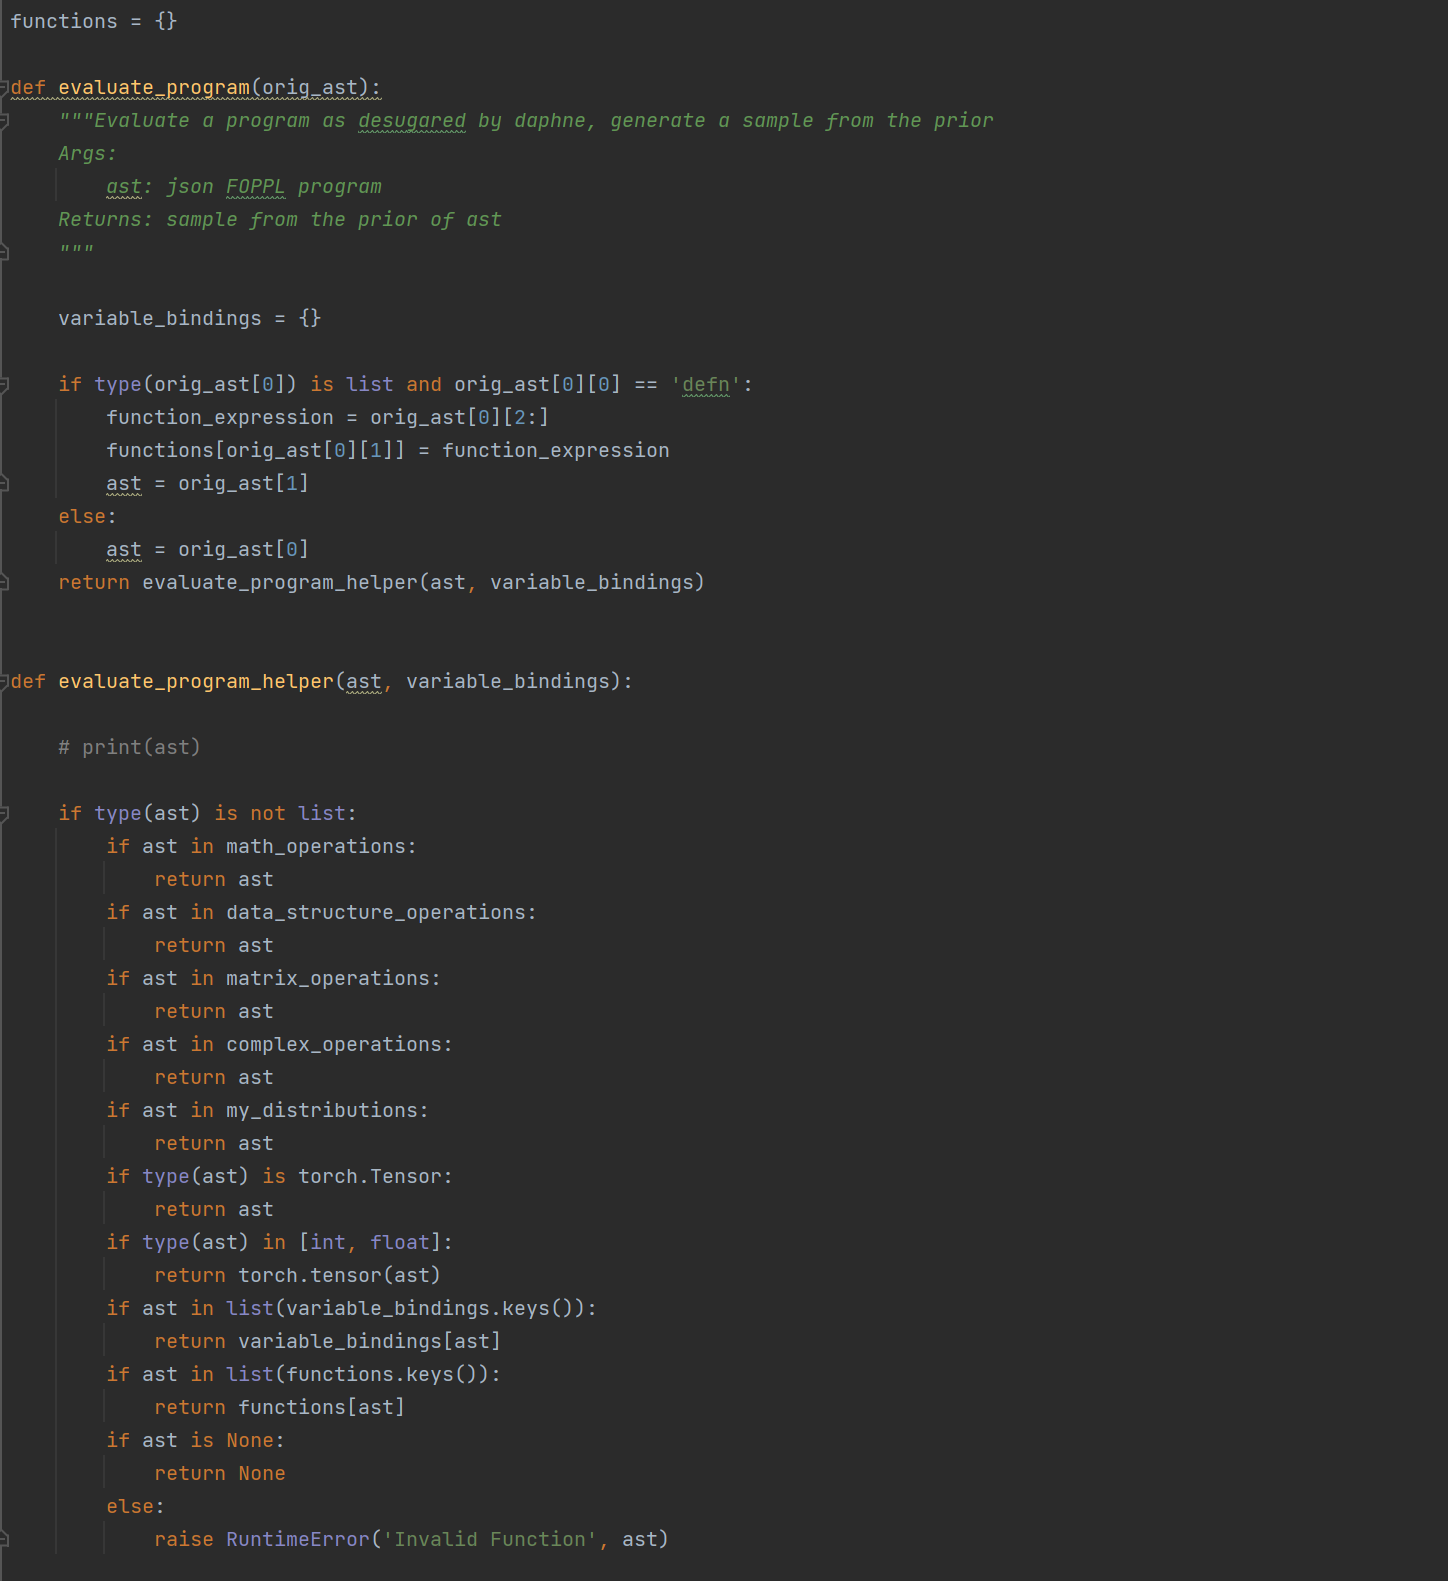
\includegraphics[scale=0.5]{figures/evaluate_program_1.png}
\end{center}

\begin{center}
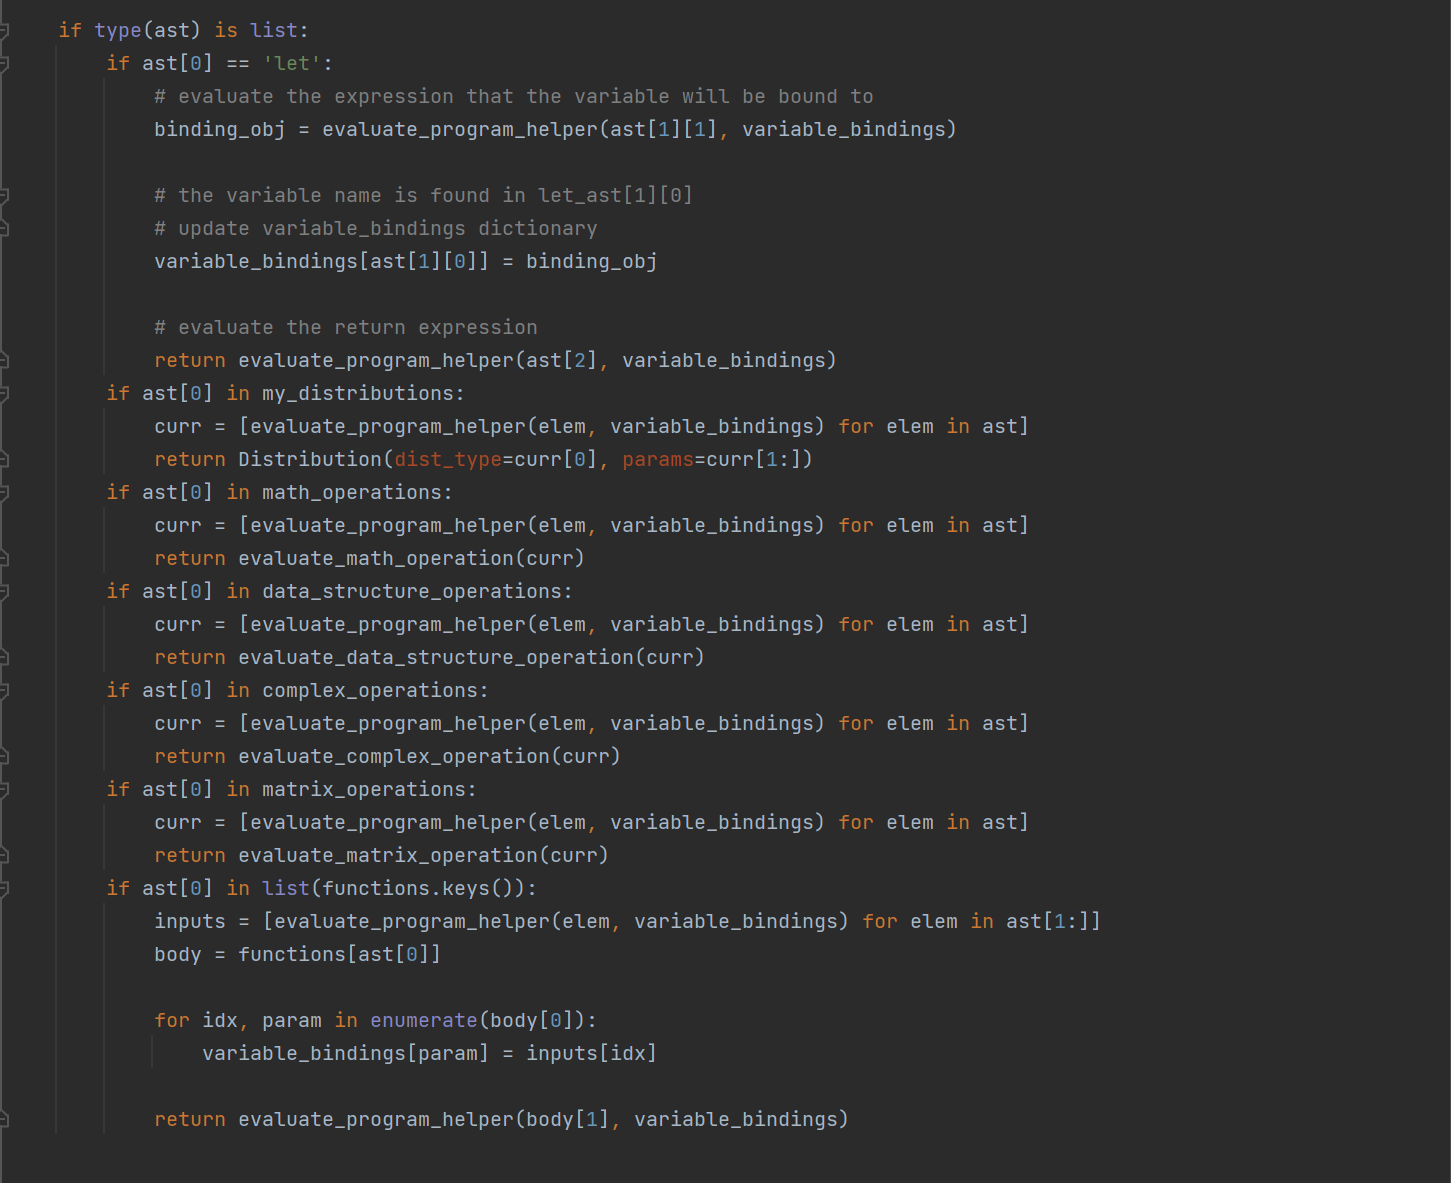
\includegraphics[scale=0.5]{figures/evaluate_program_2.png}
\end{center}

\subsection{graph\_based\_sampling.py}

\begin{center}
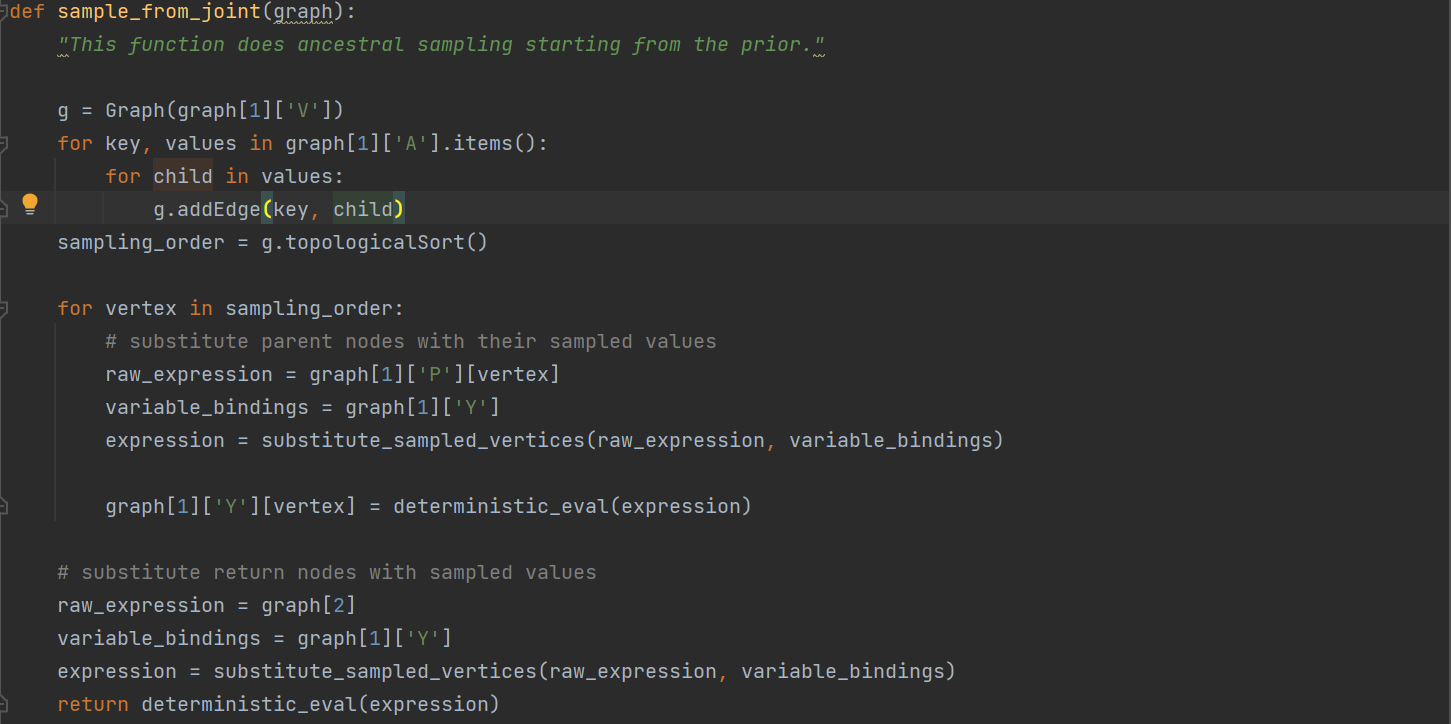
\includegraphics[scale=0.5]{figures/sample_from_joint.png}
\end{center}

\begin{center}
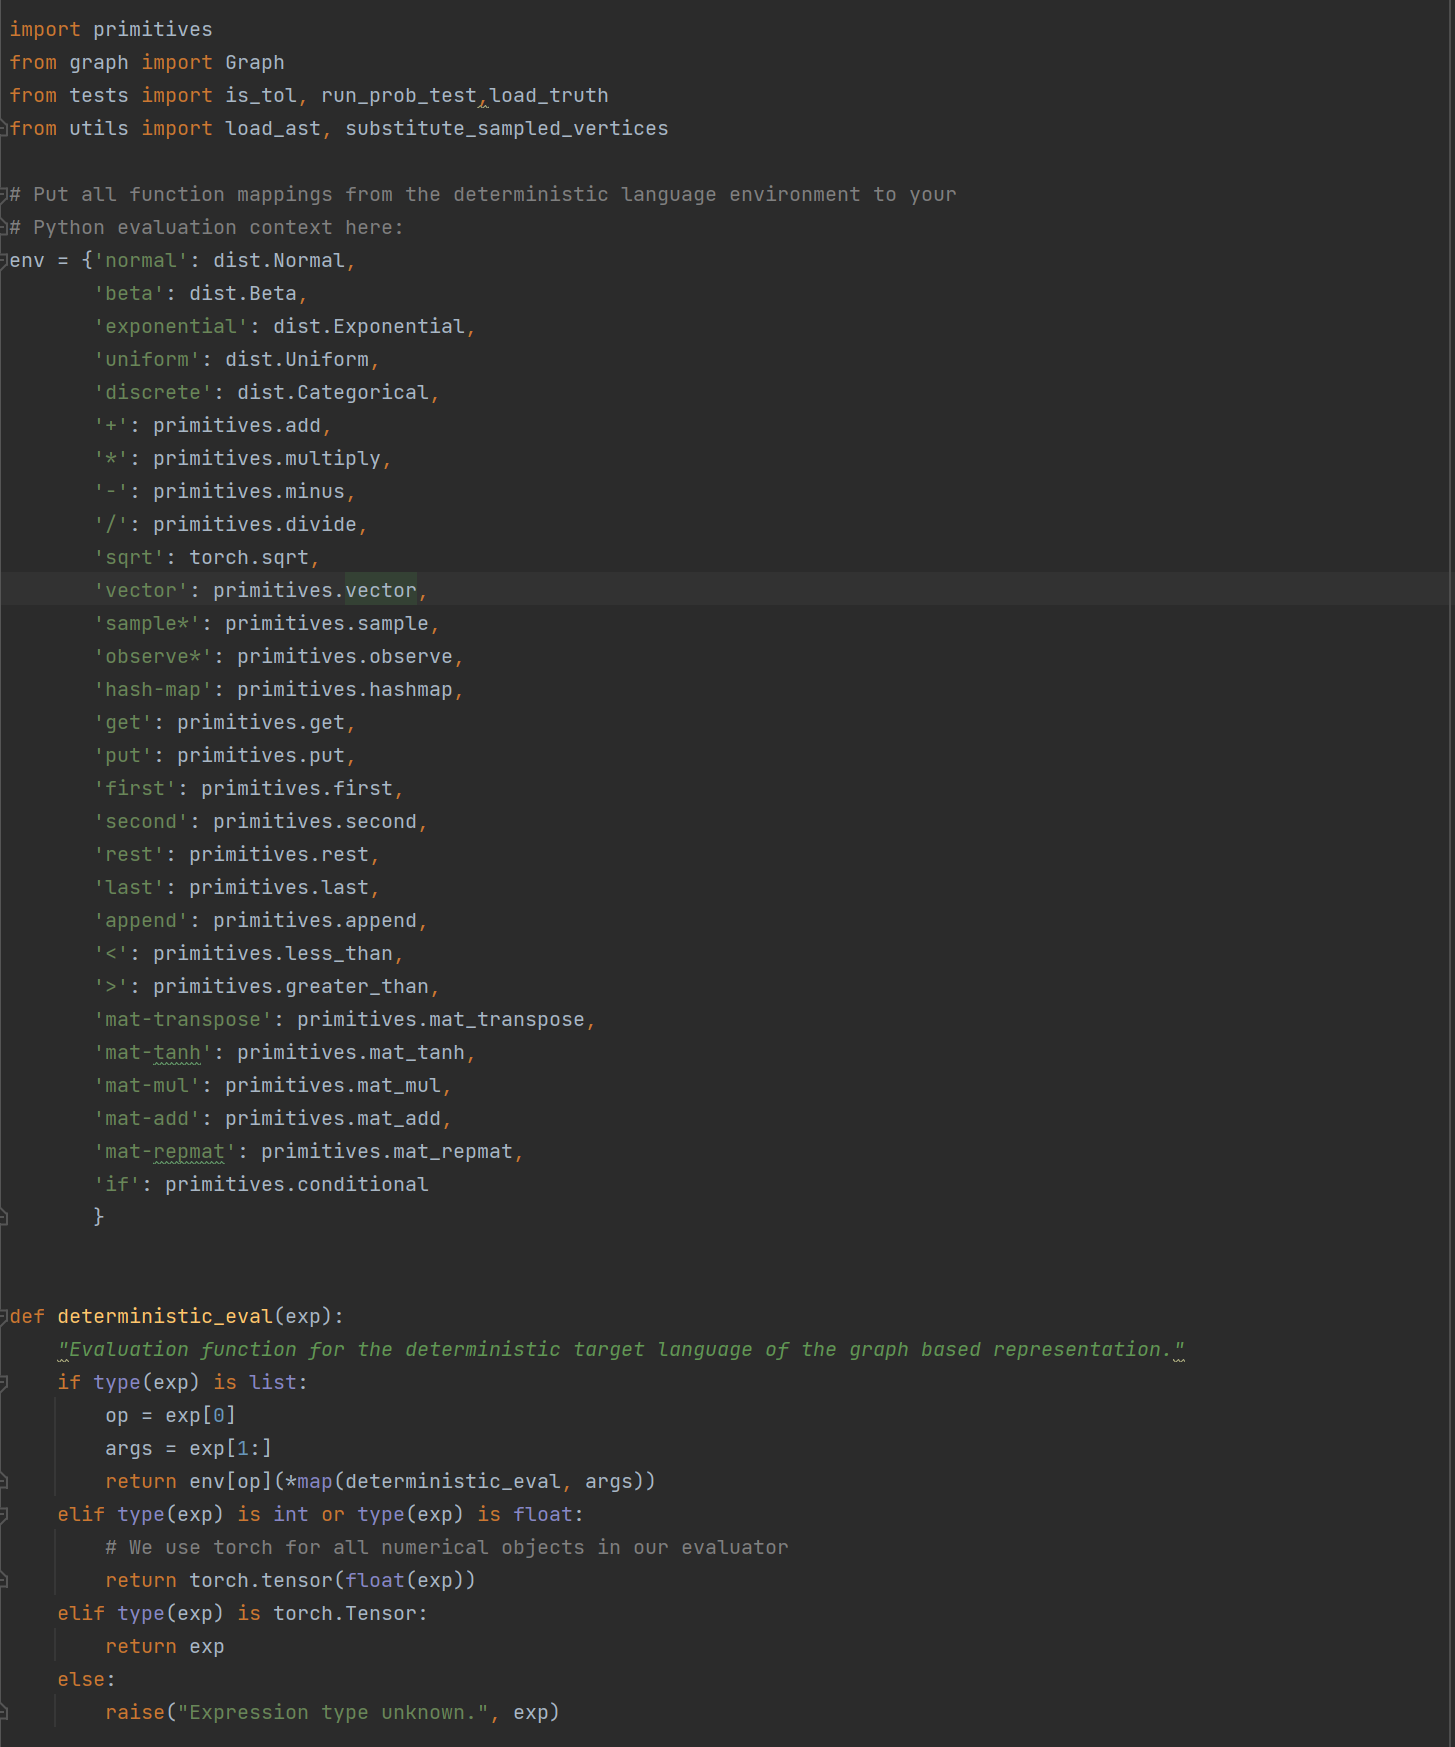
\includegraphics[scale=0.5]{figures/deterministic_eval.png}
\end{center}


\section{Unit Tests}
\subsection{Evaluation based}

\begin{center}
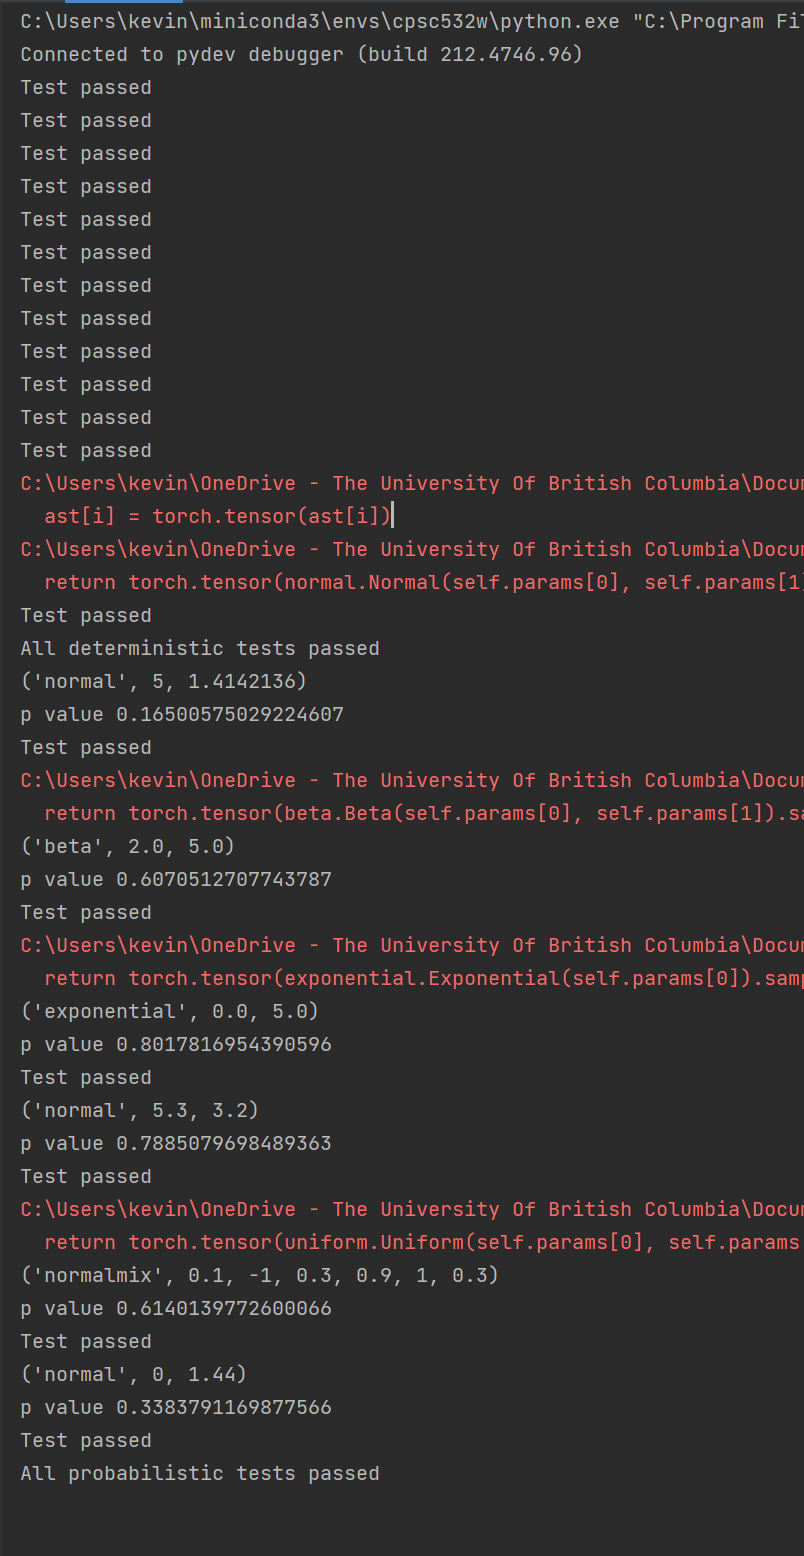
\includegraphics[scale=0.5]{figures/evaluation_unit_tests.png}
\end{center}

\subsection{Graph based}

\begin{center}
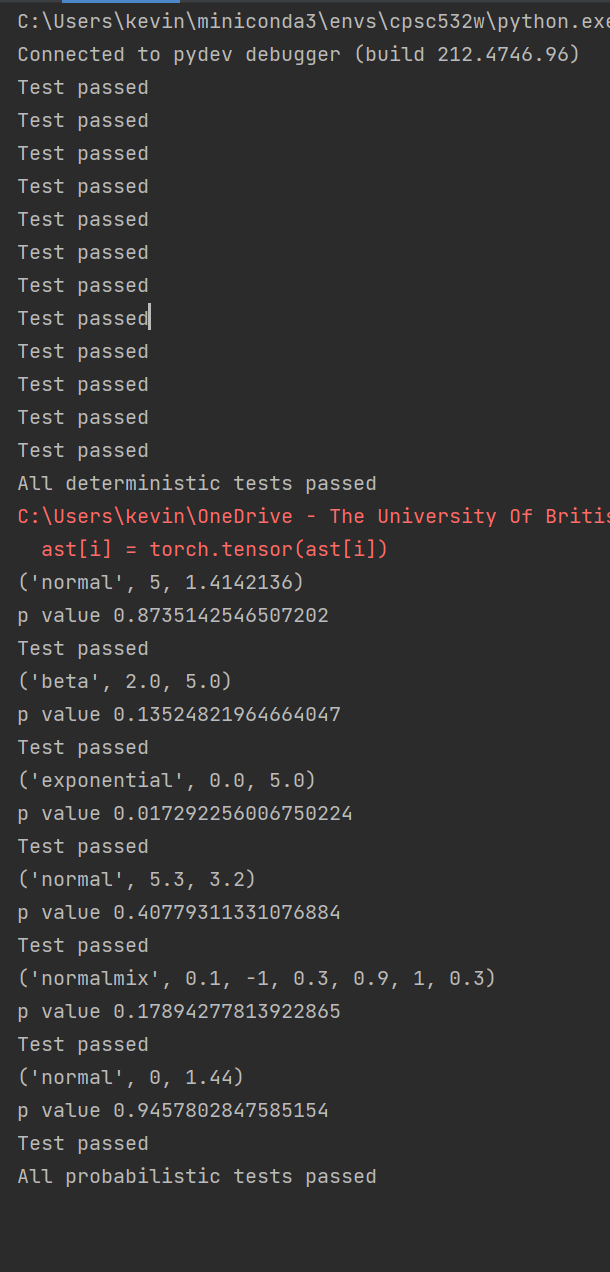
\includegraphics[scale=0.5]{figures/graph_unit_tests.png}
\end{center}


\section{Plots}

\subsection{Evaluation based}
\subsubsection{Gaussian unknown mean}
\begin{center}
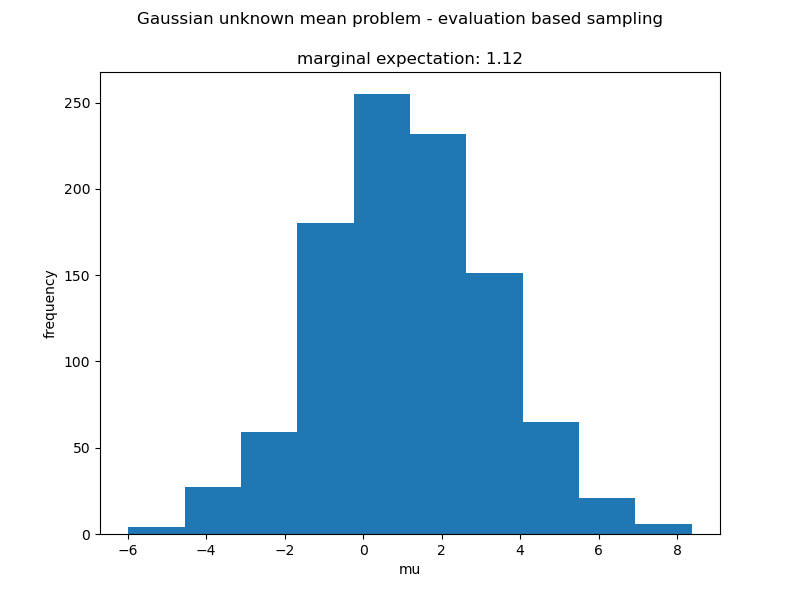
\includegraphics[scale=0.5]{figures/evaluation_1.png}
\end{center}

\subsubsection{Bayesian linear regression problem}
\begin{center}
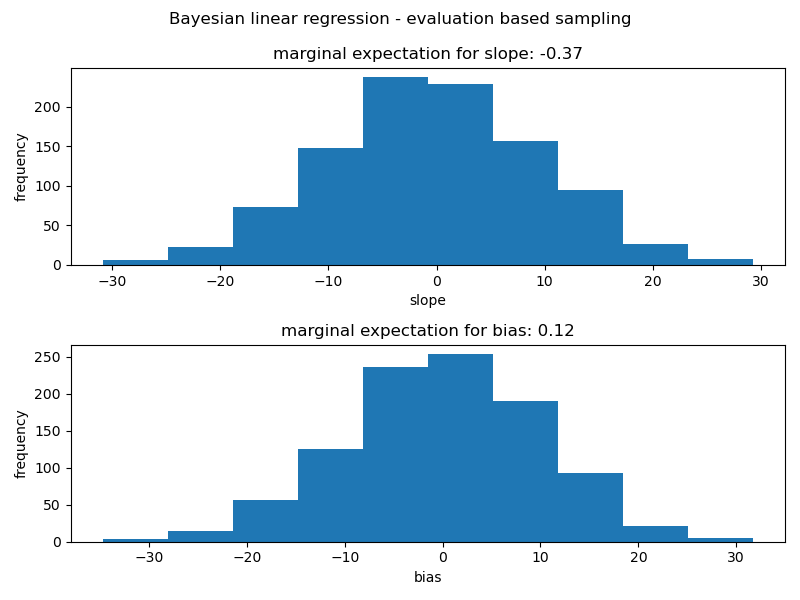
\includegraphics[scale=0.5]{figures/evaluation_2}
\end{center}

\subsubsection{Hidden Markov Model}
\begin{center}
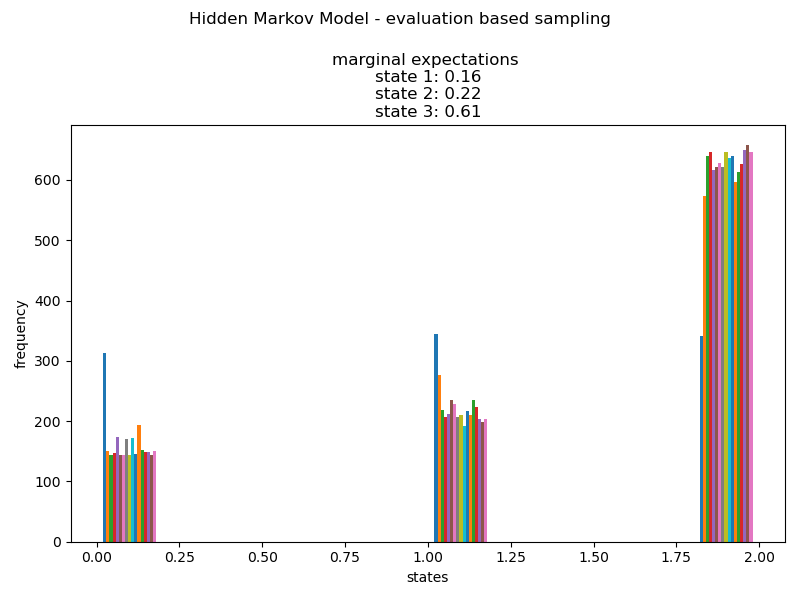
\includegraphics[scale=0.5]{figures/evaluation_3}
\end{center}

\subsubsection{Bayesian Neural Network Learning}
\begin{center}
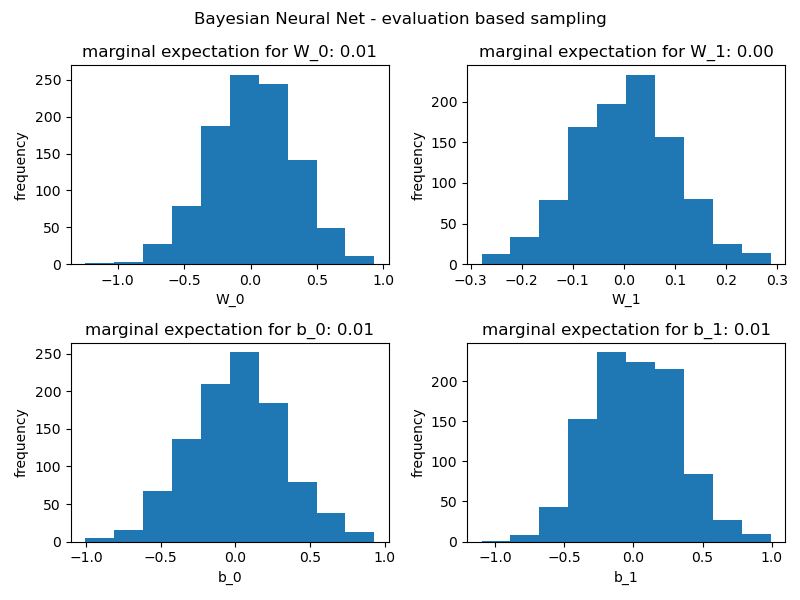
\includegraphics[scale=0.5]{figures/evaluation_4}
\end{center}


\subsection{Graph based}
\subsubsection{Gaussian unknown mean}
\begin{center}
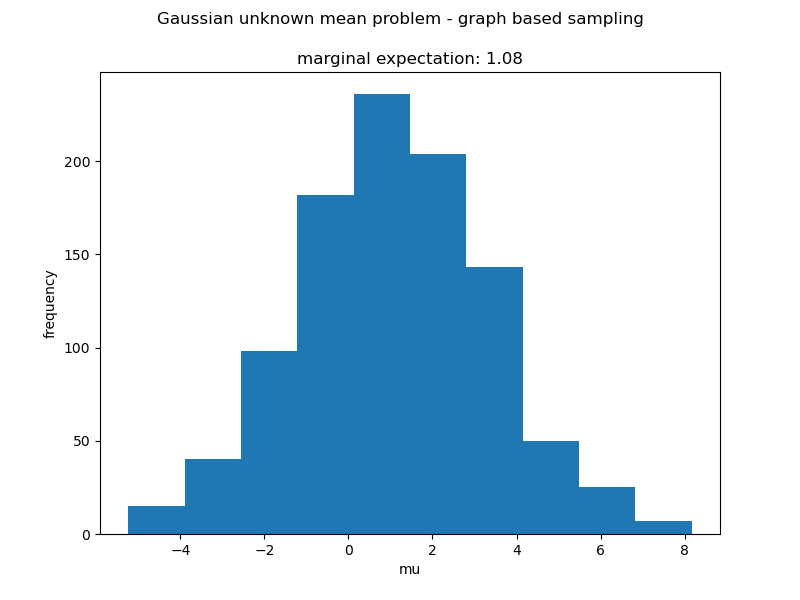
\includegraphics[scale=0.5]{figures/graph_1.png}
\end{center}

\subsubsection{Bayesian linear regression problem}
\begin{center}
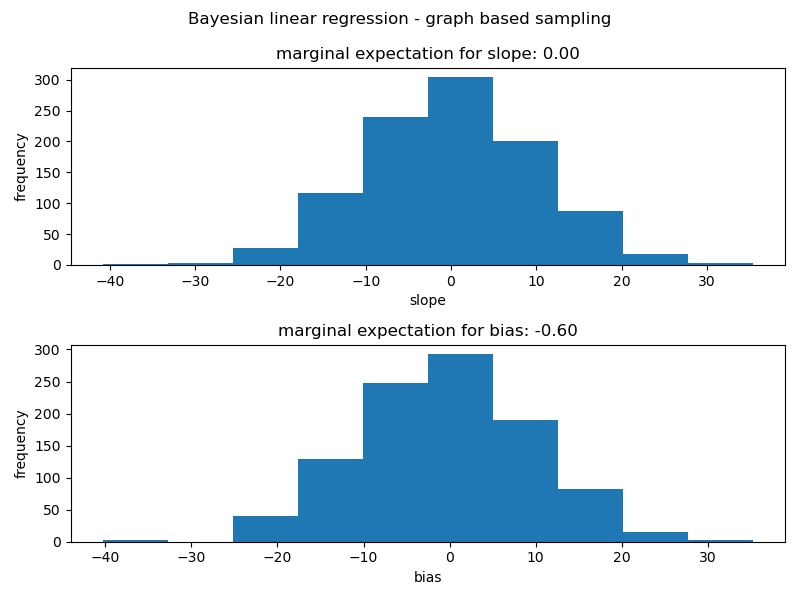
\includegraphics[scale=0.5]{figures/graph_2}
\end{center}

\subsubsection{Hidden Markov Model}
\begin{center}
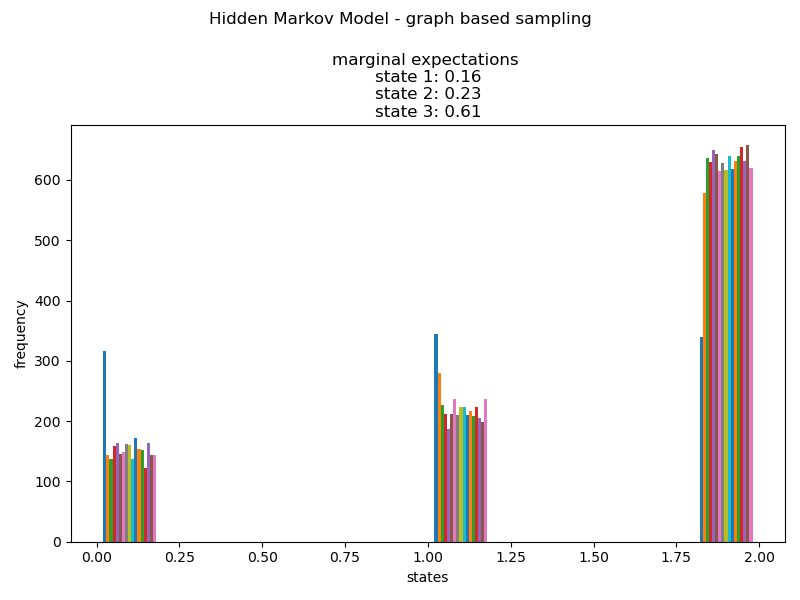
\includegraphics[scale=0.5]{figures/graph_3}
\end{center}

\subsubsection{Bayesian Neural Network Learning}
\begin{center}
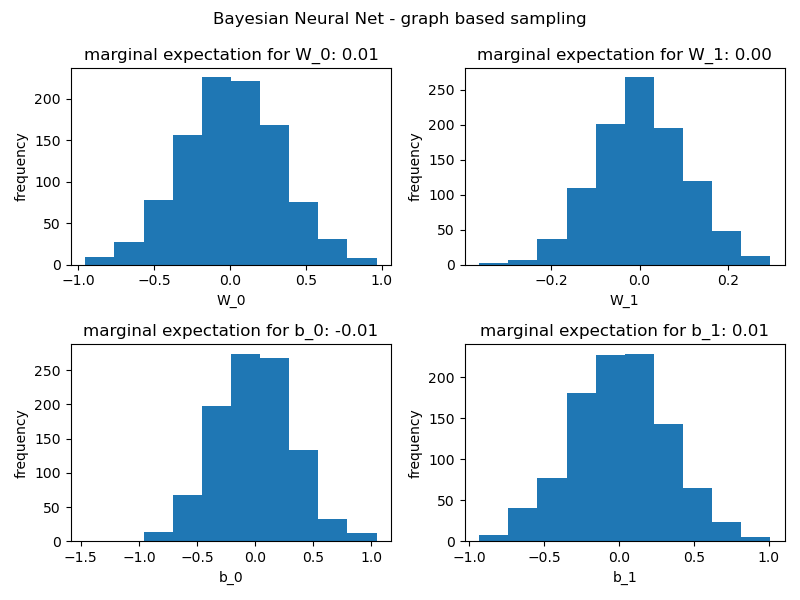
\includegraphics[scale=0.8]{figures/graph_4}
\end{center}

\end{document}